\documentclass[11pt, oneside]{article}   	% use "amsart" instead of "article" for AMSLaTeX format
\usepackage{geometry}                		% See geometry.pdf to learn the layout options. There are lots.
\geometry{letterpaper}                   		% ... or a4paper or a5paper or ... 
\usepackage{graphicx}				% Use pdf, png, jpg, or eps§ with pdflatex; use eps in DVI 
\usepackage{caption}
\usepackage{amssymb, amsmath}
\usepackage{algorithmic}
\usepackage{filecontents}

\begin{filecontents}{bibliography.bib}
@inproceedings{goodrich2010randomized,
  title={Randomized shellsort: A simple oblivious sorting algorithm},
  author={Goodrich, Michael T},
  booktitle={Proceedings of the twenty-first annual ACM-SIAM symposium on Discrete Algorithms},
  pages={1262--1277},
  year={2010},
  organization={Society for Industrial and Applied Mathematics}
}
\end{filecontents}

\title{Secure MPC Protocol for Randomized Shell Sort}
\begin{document}

\maketitle

Randomized shell sort is an oblivious sorting algorithm, developed by Michael Goodrich \cite{goodrich2010randomized}. While the paper should be referred to for a full description of the algorithm and its analysis, the following is designed to be a general introduction to the algorithm, based on its more thorough description in Goodrich\cite{goodrich2010randomized}. It additionally describes how it is implemented in JIFF in a secure manner. 

\section{Randomized Shellsort}

Recall that insertion sort is an $O(n^2)$ sorting algorithm with the following (simplified) pseudocode:

\begin{center}
\begin{algorithmic}
\STATE{Given input array $A$, let $n$ be the length of $A$ and let $B = A[0].$}
\FOR{$i$=1 to $n-1$}
	\STATE{Check each element of $B$ against $A[i]$ and insert $A[j]$ into $B$ so that the $B$ preserves its order.}
\ENDFOR
\end{algorithmic}
\end{center}

The traditional Shellsort sorting algorithm relies on the idea that insertion sort performs better on partially sorted lists. (Note, for example, that shell sort on a fully sorted list will have $O(n)$ runtime since each element only needs to be compared to the adjacent element). A traditional Shellsort algorithm uses this idea, and does a series of insertion sort algorithms on subsets of the array, where each subset is chosen by taking every ``$o^{\text{th}}$" element of the array ($o$ stands for ``offset"). In pseudocode, given array $A$ indexed from $0$ to $n-1$ and offset values $o_1,\ldots,o_p$ such that $o_i < n$, 

\begin{center}
\begin{algorithmic}
\FOR{$i=1$ to $p$}
	\FOR{$j=0$ to $o_i - 1$}
	\STATE{Sort the subarray of $A$ with indices $j, j+o_i, j+2o_i,...$ with insertion sort}
	\ENDFOR
\ENDFOR
\end{algorithmic}
\end{center}

Whether or not this is efficient depends on what series of offsets $o_1,\ldots, o_p$ is chosen. The idea behind \textit{randomized} Shellsort is to fix the offset sequence as $O = {n/2, n/4, n/8,\ldots,1}$, then compare pairs of regions $A_1$ and $A_2$ by randomly permuting the order and then doing comparisons and exchanges based on this random permutation, as shown in Fig.~\ref{fig:compare-exchange}. 

\begin{figure}
	\begin{center}
	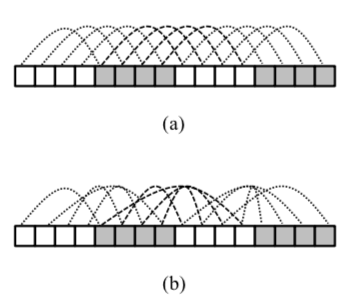
\includegraphics{compare-exchange}
	\caption{Compare-exchange operation. The dotted lines indicate the items that will be compared to one another, under (a) the identity permutation and (b) a random permutation for each pair of adjacent regions. Image from Goodrich \cite{goodrich2010randomized}.}
	\label{fig:compare-exchange}
	\end{center}
\end{figure}

Which pairs of regions are to be compared are chosen based on a schedule as follows:

\begin{figure}[!h]
	\begin{center}
	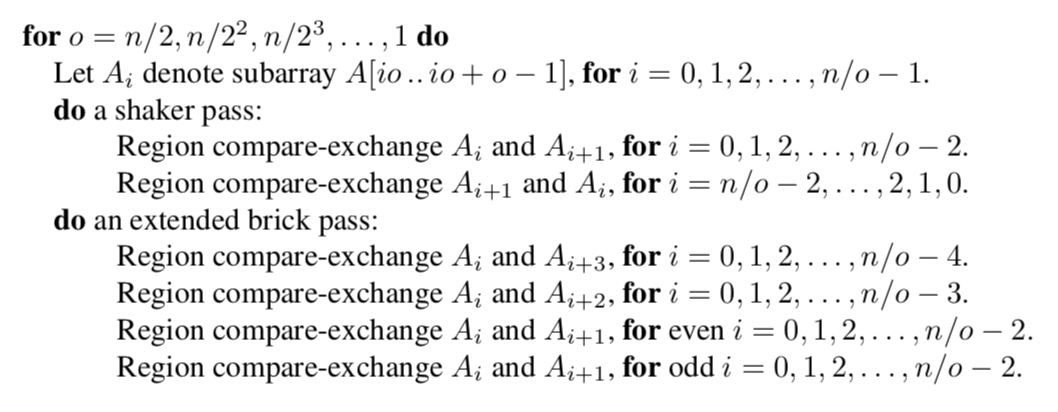
\includegraphics[scale=0.7]{shellsort}
	\caption{Randomized Shellsort pseudocode from Goodrich \cite{goodrich2010randomized}.}
	\end{center}
\end{figure}

As shown by Goodrich, this randomized Shellsort has, with high probability, a runtime of $O(n \log n)$ \cite{goodrich2010randomized}.

\section{Our Secure Implementation}

We securely implement randomized Shellsort on an array which is the element-wise sum of some number of input arrays. Since the algorithm is oblivious in the sense that everything other than the compare-exchange operation do not require knowledge of the underlying data, the majority of the algorithm may be performed without any special tools. Thus, the only portion of our implementation that requires use of the MPC library is the initial element-wise summation of the arrays and the compare-exchange operation. 

The only other nuance to this implementation is in the randomization. Since the secret-sharing that underlies the compare-exchange operations occurs in parallel for all parties, all parties must do compare-exchanges on the same elements. In other words, the random permutations that the parties do must be fixed before the computations begin. In this demo, this is handled by having the first party send out a random string to all parties, who listen for that message. All parties then use this shared random string to determine the comparisons.

\bibliographystyle{acm}
\bibliography{bibliography}
\end{document}  